% -*- coding: utf-8; -*-

\chapter{Geração Semiautomática}
\label{gordon}

	Kindlmann e Durkin foram uns dos primeiros a gerar funções de transferência para visualizar as fronteiras de um volume de dados. Apesar de ter sido publicado há quase 20 anos e de possuir alguns pontos fracos já estudado por outros, seu trabalho ainda é o mais equilibrado no quesito \quote{Geração automática \textit{X} Controle do usuário}. Isso deve-se ao fato de que seu método gera bons resultados com funções de transferência 1D, que são naturalmente mais intuitivas ao usuário. Além disso, exige intervenção mínima do usuário para gerar a FT, ao mesmo tempo que permite um controle fino sobre como a fronteira deve ser apresentada visualmente. Por esse motivo, este trabalho foi escolhido como base para a pesquisa e desenvolvimento dessa dissertação e será apresentado neste Capítulo em 4 seções. A seção~\ref{gordon.bound} define o conceito de fronteira e explica como identificá-las matematicamente. A geração da função de transferência 1D e 2D pode ser encontrada respectivamente nas seções~\ref{gordon.1d}~e~\ref{gordon.2d}. Por fim, o método é avaliado juntamente com alguns resultados, na seção~\ref{gordon.aval}.
	
\section{Detecção de fronteiras}
\label{gordon.bound}
	\textit{Kindlmann e Durkin}~\cite{gordon} partem da premissa de que todos os materiais representados no volume de dados possuem propriedades físicas homogêneas. Dessa forma, toda fronteira seria caracterizada por uma variação abrupta na intensidade lida do volume e poderia ser representada pela função degrau. No entanto, devido aos dispositivos responsáveis pela aquisição de dados, as fronteiras são comumente borradas com uma resposta gaussiana na frequência. Por esse motivo, o comportamento de uma fronteira em um volume de dados é melhor representado pela convolução da função degrau com uma gaussiana. O resultado dessa convolução é a função \textit{erf()}, ou função \textit{erro}, ilustrada na Figura~\ref{fig:boundary_model}.
	
\begin{figure}[h]
	\centering
	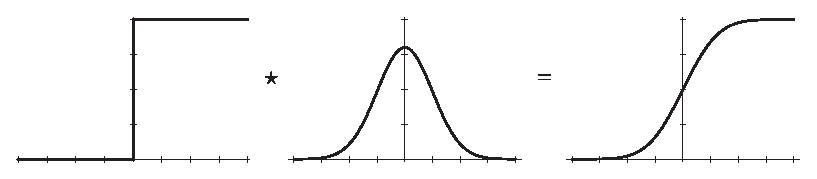
\includegraphics[width=1\textwidth]{images/g_boundary_model}
	\caption{Comportamento das funções degrau, gaussiana e erro, respectivamente~\cite{gordon}.}
	\label{fig:boundary_model}
\end{figure}

\begin{figure}[h]
	\centering
	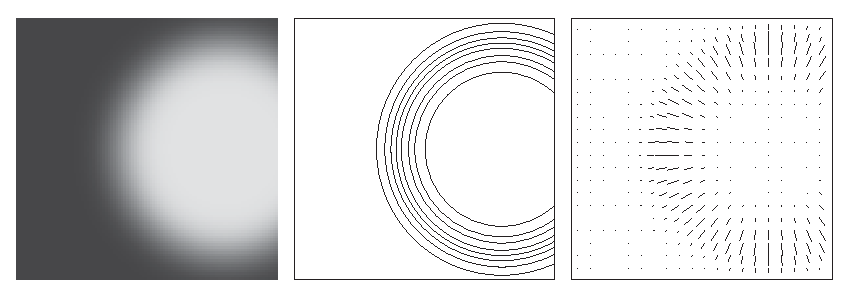
\includegraphics[width=1\textwidth]{images/grad}
	\caption{Visão em corte de um cilindro. Em~\ref{a} as intensidades do volume, em~\ref{b} as isosuperfícies e em~\ref{c} os vetores gradientes~\cite{gordon}.}
	\label{fig:grad}
\end{figure}

	Como uma fronteira pode assumir um conjunto de valores que varia entre a intensidade de dois materiais, ela pode ser interpretada como uma das isosuperfícies dentro desse conjunto de valores. Seguindo a premissa de que a fronteira é uma variação rápida de alta intensidade, ela é melhor representada pela isosuperfície que apresenta a maior derivada. Uma vez que o vetor gradiente aponta na direção da maior taxa de variação de uma função, ele pode ser usado para caminhar entre as isosuperfícies de um volume. Assim, através da avaliação da derivada na direção do gradiente, a isosuperfície que representa corretamente a fronteira entre dois isovolumes pode ser obtida.
	
	A Figura~\ref{fig:grad} ilustra algumas isosuperfícies na região de fronteira do cilindro. É possível perceber também que os gradientes se aproximam das normais das isosuperfícies, apontando sempre para uma próxima isosuperfície.
	
	A Figura~\ref{fig:functions} mostra o comportamento da primeira e segunda derivadas na presença de uma fronteira. Como esperado, o ponto de maior primeira derivada e segunda derivada igual a zero identifica a posição exata da fronteira.
	
	A função \textit{erf()} é uma função contínua cuja imagem varia de $-1$ a $1$. Como uma fronteira pode variar entre quaisquer dois valores escalares contidos no volume, \textit{erf()} deve ser escalada para variar de $s_{min}$ a $s_{max}$. Assim, a função $f(x)$ que modela uma fronteira é definida pela equação~\eqref{eq:boundary} abaixo:

\begin{equation} \label{eq:boundary}
	f(x) = s_{min} + (s_{max} - s_{min}) \frac{1 + erf(\frac{x}{\sigma\sqrt{2}})}{2}
\end{equation}
	
	A função $f$ que defina uma fronteira deveria ser definida com 3 incógnitas. Afinal, os dados estão em um espaço tridimensional. No entanto, é preciso relembrar que a curva exibida na Figura~\ref{fig:} apenas é válida na direção do gradiente. Com essa ideia em mente, a função $f$ será descrita com apenas uma incógnita, cujo eixo é sempre a direção do gradiente no ponto em que a função está sendo avaliada. Da mesma forma, como as derivadas são sempre calculadas na direção do gradiente, será omitida a direção da notação. Dessa forma, a primeira e a segunda derivada da função $f$ são, respectivamente $f'$ e $f''$.
    
\section{Função de Transferência 1D}
\label{gordon.1d}
	Texto...
    
\section{Função de Transferência 2D}
\label{gordon.2d}    
    Texto..
    
\section{Avaliação do método}
\label{gordon.aval}    
    Atacar treshold do gordon, apresentando minha solução. Mas sem criticar de forma negativa.
    
    Comentar 2ª derivada média.
    
    Como bem ressaltado por \textit{Sereda et al.}~\cite{sereda1}, é comum esperar que aumentar a dimensão da função de transferência vá trazer melhores resultados e eliminar a sobreposição de fronteiras, mas frequentemente esse não é o caso. Por esse motivo, a intuitividade em assimilar e manipular uma FT 1D foi o que motivou
    
    
    Principalmente se analisado segundo a versão 1D de sua função de transferência. Seu método trás bons resultados sem exigir intervenção do usuário. E no caso da versão 1D a interface para ser gerada e ao mesmo tempo, a versão 1D é intuitiva
    
    
    Como visto no Capítulo~\ref{related}, o trabalho de \textit{Kindlmann e Durkin}~\cite{gordon} é o que menos exige iteração do usuário para detectar fronteiras automaticamente e, ao mesmo tempo, permitindo que este possa controlar a função de transferência gerada.
    Faça uma apresentação do método....extende o trabalho relacionado + introdução e (talvez) emende nesse início de deteção de fronteira...(talvez não rs).